\section{Additional Strategy Diagnostics}
\label{app:analysis}

\subsection{Signal Similarity and Portfolio Overlap}

\begin{figure}[H]
\centering
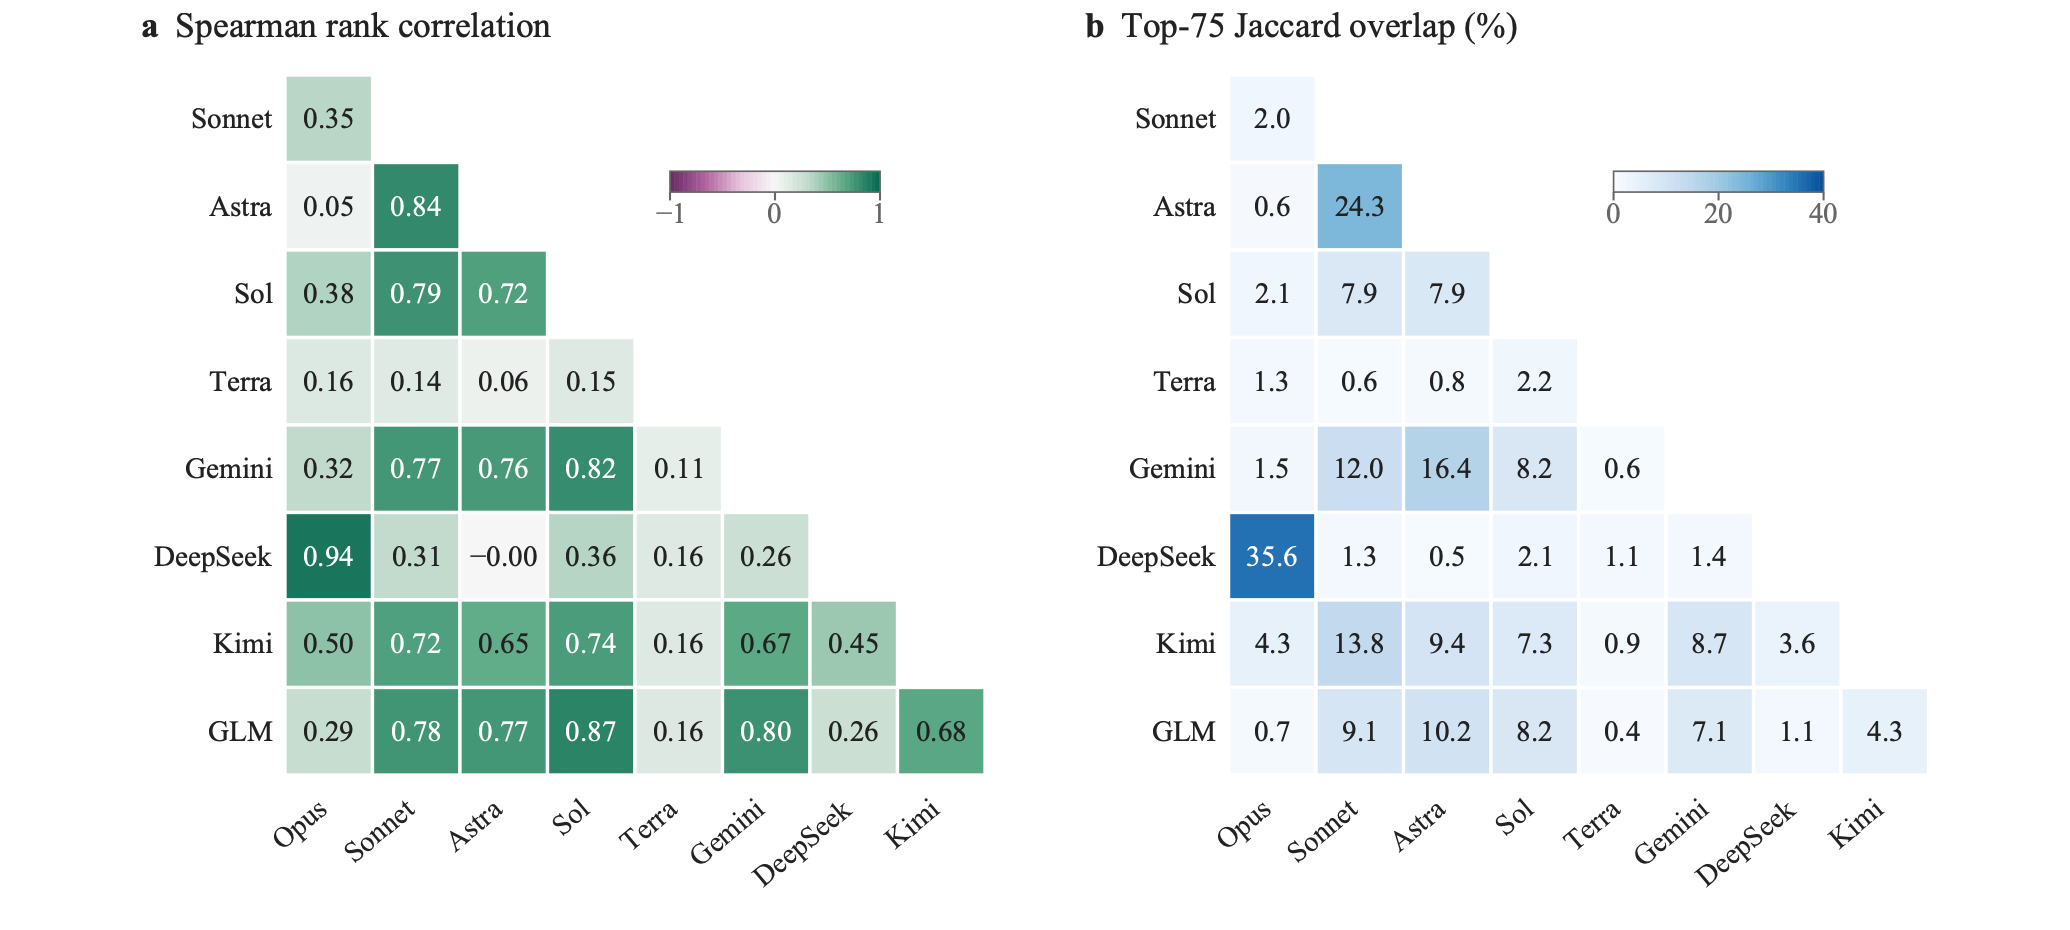
\includegraphics[width=\linewidth]{Figures/fig_similarity_r598.png}
\caption{Pairwise mean daily Spearman signal correlations (a) and Top-75 Jaccard overlaps (b) among the nine iterative representatives in 2024 (36 pairs). Portfolio overlap measures the selected score sets, rather than identical realized trades under execution constraints.}
\label{fig:similarity}
\end{figure}

The mean pairwise rank correlation is 0.47, while mean Top-75 Jaccard overlap is only 6.1\% and its maximum is 35.6\% (Figure~\ref{fig:similarity}). Broadly similar rankings therefore need not select the same extreme tail. Opus and DeepSeek are the most similar pair, with correlation 0.94 and overlap 35.6\%, followed by Sol--GLM (0.87) and Sonnet--Astra (0.84). Terra is the most distinct strategy, with a mean correlation of 0.14 against the other eight.

Opus and DeepSeek are close to each other and correlate at about 0.5 or less with every other model. This agrees with the shared tilt toward higher volatility and turnover in Figure~\ref{fig:styles}. The remaining models largely form one cluster of related signals. These similarities describe the saved signals of the nine representatives; they are not evidence that signal distinctiveness causes better returns.
